\documentclass[fleqn, a4paper, 12pt]{article}
\usepackage{amsmath, amssymb, amsthm}
\usepackage{gensymb}
\usepackage{commath}
\usepackage{xcolor}
\usepackage{cancel}
\usepackage{siunitx}
\usepackage{tikz, pgfplots}
	\usetikzlibrary{calc, hobby, patterns, intersections}
\usepackage{graphicx}
\usepackage{hyperref}
\usepackage{datetime}
\usepackage{ulem}
\usepackage{xfrac}
\usepackage{asymptote}
\usepackage{enumerate}
\setcounter{secnumdepth}{4}
\newcommand\numberthis{\addtocounter{equation}{1}\tag{\theequation}}

\newcommand{\AxisRotator}[1][rotate=0]{%
	\tikz [x=0.25cm,y=0.60cm,line width=.2ex,-stealth,#1] \draw (0,0) arc (-150:150:1 and 1);%
}

\theoremstyle{definition}
\newtheorem{example}{Example}
\newtheorem{definition}{Definition}

\theoremstyle{theorem}
\newtheorem{theorem}{Theorem}

\newenvironment{solution}
{\begin{proof}[Solution]\let\qed\relax}
	{\end{proof}}

\newcommand{\curl}{\mathrm{curl\,}}

%\renewcommand{\int_{min}^{max}}{\int\displaylimits_{min}^{max}}

%opening
\title{Lecture 22}
\author{Aakash Jog}
\date{\formatdate{13}{1}{2015}}

\begin{document}

\maketitle
%\setlength{\mathindent}{0pt}

\tableofcontents

\newpage
\section{Simple Harmonic Oscillators}

\begin{example}
	A system is arranged as follows, with the walls moving with
	\begin{align*}
		x_1 &= A \sin \omega t\\
		x_2 &= 2L + A \cos \omega t
	\end{align*}
	The entire system is in submerged in a fluid, s.t. the damping force is
	\begin{equation*}
		\overrightarrow{f} = - \beta \overrightarrow{v}
	\end{equation*}
	The mass is displaced by a small $x$ to the right. Write the equation of motion.\\
	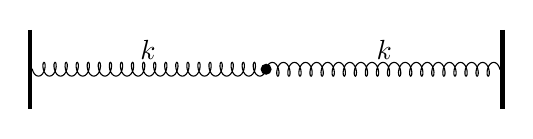
\begin{tikzpicture}
		\def\l{3};
		\def\x{0};
		\def\h{1};
		\def\segmentlength{4};
	
		\begin{scope}
			\fill (0,0) circle [radius = 2pt];
		\end{scope}
	
		\begin{scope}
			\draw [decorate, decoration = {coil, segment length = {(\l + \x)/(\l)*\segmentlength}}] (0,0) -- (\l,0) node [midway, above] {$k$};
			\draw [decorate, decoration = {coil, segment length = {(\l + \x)/(\l)*\segmentlength}}] (0,0) -- (-\l,0) node [midway, above] {$k$};
		\end{scope}
		
		\begin{scope}[ultra thick]
			\draw (-\l,{\h/2}) -- (-\l,{-\h/2});
			\draw (\l,{\h/2}) -- (\l,{-\h/2});
		\end{scope}
	\end{tikzpicture}
\end{example}

\begin{solution}
	~\\
	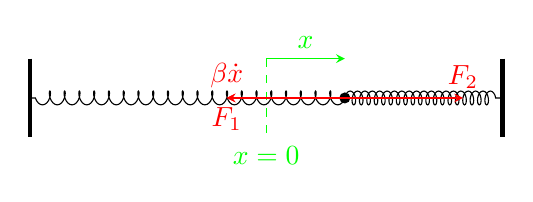
\begin{tikzpicture}
		\def\l{3};
		\def\x{1};
		\def\h{1};
		\def\F{1.5};
		\def\segmentlength{4};
		
		\coordinate (mass) at (\x,0);
		
		\begin{scope}
			\fill (mass) circle [radius = 2pt];
		\end{scope}
		
		\begin{scope}
			\draw [decorate, decoration = {coil, segment length = {(\l + -\x)/(\l)*\segmentlength}}] (mass) -- (\l,0);
			\draw [decorate, decoration = {coil, segment length = {(\l + \x)/(\l)*\segmentlength}}] (mass) -- (-\l,0);
		\end{scope}
		
		\begin{scope}[ultra thick]
			\draw (-\l,{\h/2}) -- (-\l,{-\h/2});
			\draw (\l,{\h/2}) -- (\l,{-\h/2});
		\end{scope}
		
		\begin{scope}[green]
			\draw [dashed] (0,{\h/2}) -- (0,{-\h/2}) node [below] {$x = 0$};
			\draw [-stealth] ($ (0,0) + (90:{\h/2}) $) -- ($ (mass) + (90:{\h/2}) $) node [midway, above] {$x$};
		\end{scope}
		
		\begin{scope}[red, -stealth]
			\draw (mass) -- ++(180:\F) node [above] {$\beta \dot{x}$};
			\draw (mass) -- ++(180:\F) node [below] {$F_1$};
			\draw (mass) -- ++(0:\F) node [above] {$F_2$};
		\end{scope}
	\end{tikzpicture}
	\begin{align*}
		m \ddot{x} &= -F_1 + F_2 - \beta \dot{x}\\
		&= -k(L + x - A \sin \omega t - L) + k(L - x + A \cos \omega t - L) - \beta \dot{x}
	\end{align*}
	\begin{align*}
		\therefore m \ddot{x} + \beta \dot{x} + 2 k x &= k A (\sin \omega t + \cos \omega t)\\
		\therefore \ddot{x} + \dfrac{\beta}{m} \dot{x} + \dfrac{2k}{m} x &= \dfrac{k A}{m} (\sin \omega t + \cos \omega t)
	\end{align*}
\end{solution}

\section{Coriolis Force}

\begin{tikzpicture}
	\begin{scope}[-stealth]
		\draw (0,0,0) -- (5,0,0) node [right] {$y$};
		\draw (0,0,0) -- (0,5,0) node [right] {$\overrightarrow{\omega}$};
		\draw (0,0,0) -- (0,0,5) node [below] {$x$};
	\end{scope}
	
	\begin{scope}
		\draw (0,0,0) -- (2,2,2) node [above] {$\overrightarrow{r}$};
	\end{scope}
\end{tikzpicture}

\begin{align*}
	\overrightarrow{r} &= (r \sin \theta \cos \omega t, r \sin \theta \sin \omega t, r \cos \theta)\\
	\overrightarrow{v} &= \dod{\overrightarrow{r}}{t}\\
	&= (- \omega r \sin \theta \sin \omega t, \omega r \sin \theta, 0)\\
	\overrightarrow{\omega} \times \overrightarrow{r} &= 
		\begin{vmatrix}
			\hat{x} & \hat{y} & \hat{z}\\
			0 & 0 & \omega\\
			r \sin \theta \cos \omega t & r \sin \theta \sin \omega t & r \cos \theta\\
		\end{vmatrix}\\
	&= - \omega r \sin \theta \sin \omega t \hat{x} + \omega r \sin \theta \cos \omega t \hat{y}\\
	\therefore \overrightarrow{v} &= \overrightarrow{\omega} \times \overrightarrow{r}
\end{align*}
In general, for any vector $\overrightarrow{A}$,
\begin{align*}
	\dod{\overrightarrow{A}}{t} &= \overrightarrow{\omega} \times \overrightarrow{A}
\end{align*}

%\begin{asy}[width=0.5\textwidth]
%settings.render=6;
%settings.prc=false;
%import three;
%import graph3;
%import grid3;
%currentprojection=orthographic(1,-0.175,0.33,up=Z);
%
%//Draw Axes
%pen thickblack = black+0.75;
%real axislength = 1.33;
%draw(L=Label("$x$", position=Relative(1.1), align=SW), O--axislength*X,thickblack, Arrow3); 
%draw(L=Label("$y$", position=Relative(1.1), align=N), O--axislength*Y,thickblack, Arrow3); 
%draw(L=Label("$z$", position=Relative(1.1), align=N), O--axislength*Z,thickblack, Arrow3); 
%
%//Set parameters of start corner of polar volume element
%real r = 1;
%real q=0.3pi; //theta
%real f=0.35pi; //phi
%
%real dq=0.15; //dtheta
%real df=0.3; //dphi
%real dr=0.1; 
%
%
%// Arq is A + dr*rhat + dq*qhat, etc
%triple A = r*expi(q,f);
%triple Ar = (r+dr)*expi(q,f);
%triple Aq = r*expi(q+dq,f);
%triple Arq = (r+dr)*expi(q+dq,f);
%triple Af = r*expi(q,f+df);
%triple Arf = (r+dr)*expi(q,f+df);
%triple Aqf = r*expi(q+dq,f+df);
%triple Arqf = (r+dr)*expi(q+dq,f+df);
%
%pen thingray = gray+0.33;
%
%draw(A--Ar);
%draw(Aq--Arq);
%draw(Af--Arf);
%draw(Aqf--Arqf);
%draw( arc(O,A,Aq) ,thickblack );
%draw( arc(O,Af,Aqf),thickblack );
%draw( arc(O,Ar,Arq) );
%draw( arc(O,Arf,Arqf) );
%draw( arc(O,Ar,Arq) );
%draw( arc(O,A,Af),thickblack );
%draw( arc(O,Aq,Aqf),thickblack );
%draw( arc(O,Ar,Arf) );
%draw( arc(O,Arq,Arqf) );
%
%pen thinblack = black+0.25;
%
%//phi arcs
%draw(O--expi(pi/2,f),thinblack);
%draw("$\varphi$", arc(O,0.5*X,0.5*expi(pi/2,f)),thinblack,Arrow3);
%draw(O--expi(pi/2,f+df),thinblack);
%draw( "$d\varphi$", arc(O,expi(pi/2,f),expi(pi/2,f+df) ),thinblack );
%draw( A.z*Z -- A,thinblack);
%draw(L=Label("$r\sin{\theta}$",position=Relative(0.5),align=N), A.z*Z -- Af,thinblack);
%
%//cotheta arcs
%draw( arc(O,Aq,expi(pi/2,f)),thinblack );
%draw( arc(O,Aqf,expi(pi/2,f+df) ),thinblack);
%
%//theta arcs
%draw(O--A,thinblack);
%draw(O--Aq,thinblack);
%draw("$\theta$", arc(O,0.25*length(A)*Z,0.25*A),thinblack,Arrow3);
%draw(L=Label("$d\theta$",position=Relative(0.5),align=NE) ,arc(O,0.66*A,0.66*Aq),thinblack );
%
%
%// inner surface
%triple rin(pair t) {  return r*expi(t.x,t.y);}
%surface inner=surface(rin,(q,f),(q+dq,f+df),16,16);
%draw(inner,emissive(gray+opacity(0.33)));
%//part of a nearly transparent sphere to help see perspective
%surface sphere=surface(rin,(0,0),(pi/2,pi/2),16,16);
%draw(sphere,emissive(gray+opacity(0.125)));
%
%
%// dr and rdtheta labels
%draw(L=Label("$dr$",position=Relative(1.1)), Af + 0.5*(Arf-Af)--Af + 0.5*(Arf-Af)+0.25*Z,dotted);
%triple U=expi(q+0.5*dq,f);
%draw(L=Label("$rd\theta$",position=Relative(1.1)), r*U ---r*(1.33*U.x,1.33*U.y,U.z),dotted );
%
%\end{asy}

The system $S : x y z$ is inertial, and the system $S' : x' y' z'$ is rotating around $\overrightarrow{\omega}$ relative to $S$.\\
Therefore, the position vector $\overrightarrow{r}$ can be written as follows.
\begin{align*}
	\overrightarrow{r} &= x \hat{x} + y \hat{y} + z \hat{z}\\
	\overrightarrow{r'} &= x' \hat{x'} + y' \hat{y'} + z' \hat{z'}	
\end{align*}
Therefore,
\begin{align*}
	\overrightarrow{v} &= \dot{x} \hat{x} + \dot{y} \hat{y} + \dot{z} \hat{z}\\
	\overrightarrow{v'} &= \dot{x}' \hat{x'} + \dot{y}' \hat{y'} + \dot{z}' \hat{z'}\\
	\overrightarrow{a} &= \ddot{x} \hat{x} + \ddot{y} \hat{y} + \ddot{z} \hat{z}\\
	\overrightarrow{a'} &= \ddot{x}' \hat{x'} + \ddot{y}' \hat{y'} + \ddot{z}' \hat{z'}
\end{align*}
Therefore, in $S$,
\begin{align*}
	\overrightarrow{v} &= \dod{\overrightarrow{r}}{t}\\
	&= \dod{\overrightarrow{r'}}{t}\\
	&= \dot{x'} \hat{x'} + \dot{y'} \hat{y'} + \dot{z'} \hat{z'}\\
	&\quad + x' \dod{\hat{x'}}{t} + y' \dod{\hat{y'}}{t} + z' \dod{\hat{z'}}{t}\\
	&= \overrightarrow{v'} + x' \left( \overrightarrow{\omega} \times \hat{x'} \right) + y' \left( \overrightarrow{\omega} \times \hat{y'} \right) + z' \left( \overrightarrow{\omega} \times \hat{z'} \right)\\
	&= \overrightarrow{v'} + \overrightarrow{\omega} \times \left( x' \hat{x'} + y' \hat{y'} + z' \hat{z'} \right)\\
	&= \overrightarrow{v'} + \overrightarrow{\omega} \times \overrightarrow{r}
\end{align*}
Similarly,
\begin{align*}
	\overrightarrow{a} &= \dod{}{t} \left( \overrightarrow{v'} + \overrightarrow{\omega} \times \overrightarrow{r} \right)\\
	&= \dod{\overrightarrow{v'}}{t} + \overrightarrow{\omega} \times \dod{\overrightarrow{r}}{t}\\
	&= \dod{}{t} \left( \dot{x}' \hat{x'} + \dot{y}' \hat{y'} + \dot{z}' \hat{z'} \right) + \overrightarrow{\omega} \times \left( \overrightarrow{v'} + \overrightarrow{\omega} \times \overrightarrow{r} \right)\\
	&= \ddot{x'} \hat{x'} + \dot{x'} \dod{\hat{x'}}{t} + \ddot{y'} \hat{y'} + \dot{y'} \dod{\hat{y'}}{t} + \ddot{z'} \hat{z'} + \dot{z'} \dod{\hat{z'}}{t}\\
	&\quad + \overrightarrow{\omega} \times \overrightarrow{v'} + \overrightarrow{\omega} \times \left( \overrightarrow{\omega} \times \overrightarrow{r} \right)\\
	&= \overrightarrow{a'} + 2 \overrightarrow{\omega} \times \overrightarrow{v'} + \overrightarrow{\omega} \times \left( \overrightarrow{\omega} \times \overrightarrow{r} \right)
\end{align*}
Therefore,
\begin{equation*}
	m \overrightarrow{a'} = \underbrace{m \overrightarrow{a}}_{\sum \overrightarrow{F}} - \underbrace{2 m \overrightarrow{\omega} \times \overrightarrow{v}}_{\text{coriolis force}} - \underbrace{m \overrightarrow{\omega} \times \left( \overrightarrow{\omega} \times \overrightarrow{r} \right)}_{\text{centrifugal force}}
\end{equation*}

\begin{example}
	Find the forces acting on a body at a small distance above the surface of the earth, at angle $\lambda$ from the equator, moving with $\omega$.\\
\end{example}

\begin{solution}
	\begin{tikzpicture}
		\def\R{4};
		\def\h{1};
		\def\angle{30};
		\def\F{2};
		
		\coordinate (mass) at (\angle:{\R + \h});
		
		\draw (0,0) circle [radius = \R];
		
		\fill (mass) circle [radius = 2pt];
		
		\begin{scope}[-stealth]
		\draw (mass) -- ++({180 + \angle}:\F) node [below] {$mg$};
		\draw (mass) -- ++(0:\F) node [below] {$m \omega^2 R \cos \lambda$};
		\end{scope}
		
		\node [above] at (mass) {$2 m \omega v \cos \lambda \otimes$};
		
		\draw [dashed] (0,0) -- ++(\angle:\R);
		\draw [dashed] (0,0) -- ++(0:\R) node [midway, fill = white] {$R$};
		
		\node at ({\angle/2}:1) {$\lambda$};
	\end{tikzpicture}
\end{solution}

\begin{example}
	A disk with a diametrical partition is rotating anti-clockwise with $\omega$, as shown. Two small masses start moving with $v_0$ as shown. Which ball moves away from the partition?\\
	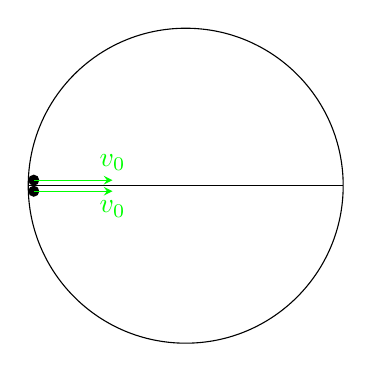
\begin{tikzpicture}
		\def\R{2};
		\def\F{1};
		
		\coordinate (m1) at (2pt,2pt);
		\coordinate (m2) at (2pt,-2pt);
		
		\draw (\R,0) circle [radius = \R];
		
		\draw (0,0) -- (2*\R,0);
		
		\fill (m1) circle [radius = 2pt];
		\fill (m2) circle [radius = 2pt];
		
		\begin{scope}[green, -stealth]
			\draw (m1) -- ++(0:\F) node [above] {$v_0$};
			\draw (m2) -- ++(0:\F) node [below] {$v_0$};
		\end{scope}
	\end{tikzpicture}
\end{example}

\begin{solution}
	~\\
	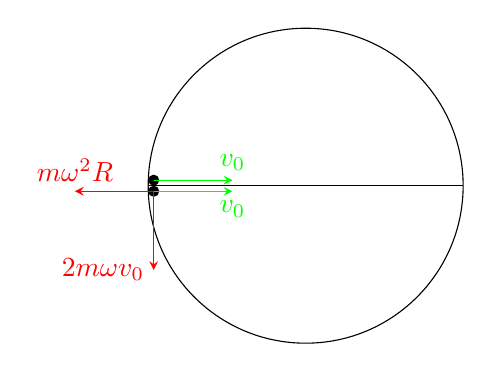
\begin{tikzpicture}
		\def\R{2};
		\def\F{1};
		
		\coordinate (m1) at (2pt,2pt);
		\coordinate (m2) at (2pt,-2pt);
		
		\draw (\R,0) circle [radius = \R];
		
		\draw (0,0) -- (2*\R,0);
		
		\fill (m1) circle [radius = 2pt];
		\fill (m2) circle [radius = 2pt];
		
		\begin{scope}[green, -stealth]
		\draw (m1) -- ++(0:\F) node [above] {$v_0$};
		\draw (m2) -- ++(0:\F) node [below] {$v_0$};
		\end{scope}
		
		\begin{scope}[red, -stealth]
		\draw (m2) -- ++(180:\F) node [above] {$m \omega^2 R$};
		\draw (m2) -- ++(-90:\F) node [left] {$2 m \omega v_0$};
		\end{scope}
	\end{tikzpicture}\\
	Therefore, the ball which is below the partition moves away from the partition.
\end{solution}

\end{document}